\documentclass[10 pt,usenames,dvipsnames, oneside]{article}
\usepackage{../../modelo-fracoes}
\graphicspath{{../../../Figuras/licao01/}}


\begin{document}

\begin{center}
  \begin{minipage}[l]{3cm}

\includegraphics[width=2cm]{../../../Figuras/logo}       
\end{minipage}\hfill
\begin{minipage}[r]{.8\textwidth}
 {\Large \scshape Atividade: Repartindo um chocolate em três partes}  
\end{minipage}
\end{center}
\vspace{.2cm}

\ifdefined\prof
\begin{goals}

\begin{enumerate}

\item[OE1] Diferenciar a partição da unidade em partes “quaisquer”
da partição da unidade em partes “iguais”.
\item[OE2] Reconhecer a necessidade de uma expressão verbal
que identifique uma das partes iguais em uma equipartição
da unidade.
\item[OE3] Diferenciar “a partição da unidade em três partes
quaisquer” da “partição da unidade em três partes
iguais”.
\item[OE4] Compreender as expressões “um terço de” e “terça
parte de” como formas de identificar uma das partes da
equipartição da unidade em três partes.

\end{enumerate}

\tcblower

\begin{itemize}
\item No final deste volume estão disponíveis materiais para
reprodução. Mas o professor pode usar folhas de papel
para o mesmo fim.
\item Recomenda‐se que a atividade seja desenvolvida em
grupos de 3 a 5 alunos.
\item A partição em partes iguais será chamada neste texto
de “equipartição”, mas consideramos desnecessário o
uso desta palavra pelo professor com os estudantes. O
objetivo é fazer a equipartição livremente de forma coerente.
Assim, por exemplo, podem ser aceitas como
respostas:
\begin{center}
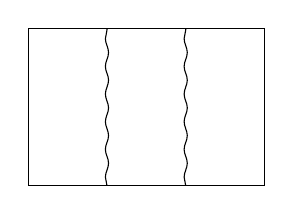
\begin{tikzpicture}[x=1cm, y=1cm]
\draw (0,0) rectangle (3,2);
\draw[decorate, decoration={snake, amplitude= .2 mm}] (1,0) -- (1,2);
\draw[decorate, decoration={snake, amplitude= .2 mm}] (2,0) -- (2,2);        
\end{tikzpicture}
\end{center}
\item Não se espera que, nesta atividade, os alunos usem a
medida para fazer a equipartição de maneira precisa.
\item Busque conduzir a discussão nos grupos de modo que
os estudantes percebam que, para que os amigos recebam
a mesma quantidade de chocolate, a partição proposta
para a barra de chocolate deve ser em “partes
iguais”, no sentido de ganharem todos a mesma quantidade
de chocolate, não necessariamente pedaços de
mesma forma.
\item Na discussão, procure destacar que a referência à
“partição em três partes iguais” se dá a partir das expressões
“um terço” da barra de chocolate ou “a terça
parte” da barra de chocolate.
\item item c) admite diversas soluções, algumas estão
apresentadas como resposta. No entanto, algumas dessas
respostas podem não aparecer naturalmente em sala
de aula. Avalie a possibilidade de apresentar e explorar
algumas dessas soluções (ou outras que queira) em sala
de aula. Por exemplo, apresente uma dessas divisões
aos alunos e peça‐lhes que avaliem a equipartição, explicando
sua decisão.
\item O item d), provavelmente, pode não ser respondido corretamente pelos alunos. Se for o caso, as expressões ``um terço de'' e ``a terça parte de'' devem ser apresentadas.
\item Fique atento às falas dos alunos. Observe que os alunos podem representar e verbalizar as respostas de diferentes modos e que não há uma resposta única para a atividade. Por exemplo, alguns alunos podem precisar de mais tempo do que outros para usar a expressão       ``um terço'' no lugar de       ``partição em três partes iguais'' ou ``divisão em três partes iguais''. Ou ainda, observarem que há diferentes representações para a equipartição.
\item Pode ser aproveitada a oportunidade para questionar os estudantes se no lugar de três amigos fossem 5 amigos, cada um receberia mais ou menos chocolate após a divisão em cinco partes iguais?
\item Esta atividade pode ser adaptada visando a inclusão de alunos com deficiência de visão. Para isso, sugere-se confeccionar os modelos da barra de chocolate  inteira e repartida, que estão disponíveis para reprodução no final do livro, em três materiais diferentes. Por exemplo, papel comum e papéis com texturas diferentes, tecido ou material emborrachado.
\end{itemize}

\end{goals}

\bigskip
\begin{center}
{\large \scshape Atividade}
\end{center}
\fi

Três amigos repartiram uma barra de chocolate. Veja como eles fizeram.

  \begin{center}
    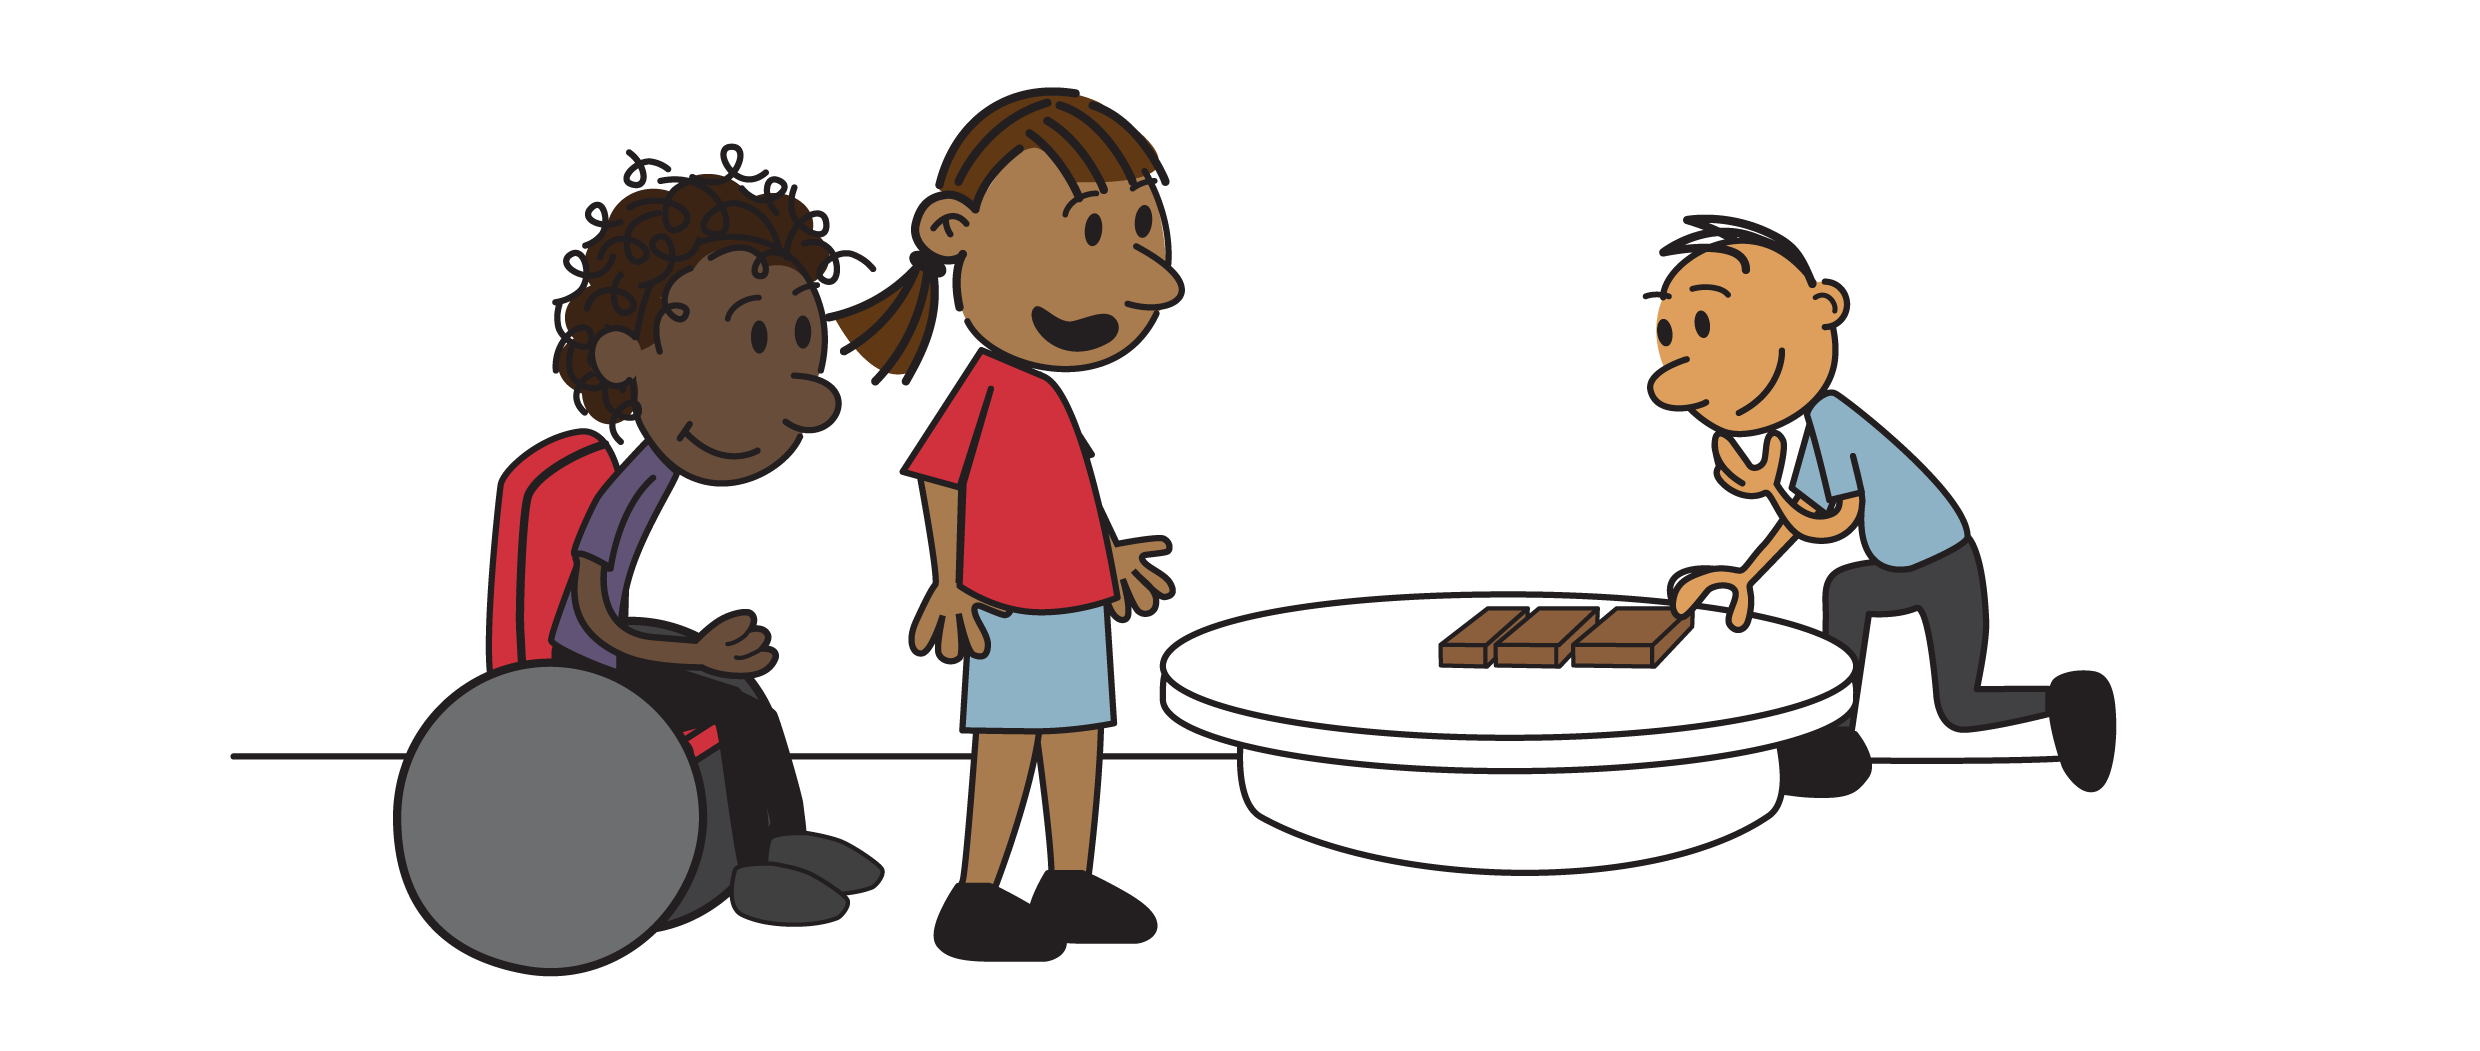
\includegraphics[width=300pt, keepaspectratio]{ativ1_fig01.png}
  \end{center}

\begin{enumerate}[label=\alph*)] %s
  \item Você concorda com essa divisão? Explique.
  \item Com essa divisão, os três amigos receberam a mesma quantidade de chocolate?
  \item Desenhe uma divisão da barra de chocolate que permita que os 3 amigos recebam quantidades iguais de chocolate.

    \begin{center}
      
\begin{tikzpicture}[scale=10]
 \draw[fill={rgb,255:red,141; green,94; blue,66}] (0,0) rectangle (4.5,2);        
      \end{tikzpicture}
    \end{center}

  \item Considerando a divisão da barra de chocolate em 3 partes iguais, como você nomearia a quantidade de chocolate que cada amigo receberia?
\end{enumerate} %s

\ifdefined\prof

\begin{solucao}

\begin{enumerate}[label=\alph*),wide,labelindent=0pt] %s
    \item       Este item não possui resposta correta, apenas respostas coerentes com a explicação do aluno. Por exemplo, um estudante pode dizer que sim e explicar que o amigo mais velho deve ficar com uma parte maior porque precisa de mais energia. Mas a resposta esperada é que a divisão não parece justa porque as quantidades de chocolate são diferentes. Discuta com os alunos para que entendam a divisão correspondente à resposta esperada.
    \item Não, eles receberão quantidades diferentes de chocolate, embora cada um receba um único pedaço do chocolate.
    \item Respostas possíveis:

\begin{center}
  \begin{tikzpicture}[scale=10,every path/.style={black}]
   \draw (0,0) rectangle (3,2);
   \draw (1,0) -- (1,2);
   \draw (2,0) -- (2,2);
  \end{tikzpicture}
  \begin{tikzpicture}[scale=10,every path/.style={black}]
   \draw (0,0) rectangle (3,2);
   \draw (0,.6666) -- (3,.6666);
   \draw (0,1.3333) -- (3,1.3333);
  \end{tikzpicture}
  \begin{tikzpicture}[scale=10,every path/.style={black}]
   \draw (0,0) rectangle (3,2);
   \draw (0,1.3333) -- (3,1.3333);
   \draw (1.5,0) -- (1.5,1.333);
  \end{tikzpicture}
  \begin{tikzpicture}[scale=10,every path/.style={black}]
   \draw (0,0) rectangle (3,2);
   \draw (1,0) -- (1,2);
   \draw (1,1) -- (3,1);
  \end{tikzpicture}
\end{center}
  %\noindent\includegraphics[width=.45\textwidth, keepaspectratio]{../..//media/cap1/secoes/licao1_atv1.png}
    \item       Cada parte é {\it um terço} da barra ou a {\it terça parte} da barra.
\end{enumerate} %s

\end{solucao}
\fi

\end{document}